%!tex root = ../main.tex

%\section{Automatically proving lower bounds for LCL problems} \label{sec:implementation}
\section{Implementation} \label{sec:implementation}
In this section we will cover all the important topics that are used in the actual implementation of the Algorithm \ref{alg:counterexample_finder} from Section \ref{sec:algorithm}.
This includes the previously declared functions $\textsc{IsUnsolvable}(\Pi, g)$ and $\textsc{GenerateGraphs}(n, d_a, d_p)$, which were given as black boxes.
The implementation itself is a computer program, that attempts to automatically find a proof of unsolvability for a given LCL problem in PN model.
We keep the explanations independent of any programming language, so that the reader can understand these upcoming topics without needing such knowledge.
% (see section \ref{sec:port-numbering_model} for more information about PN model).

The function $\textsc{IsUnsolvable}(\Pi, g)$ checks if an LCL problem $\Pi$ is unsolvable in some $(d_a, d_p)$-biregular multigraph $g$.
To perform the checking, it is enough to show that there exists no valid labeling of $\Pi$ in $g$.
In the implementation this is done with following steps:
\begin{enumerate}
    \item encode the problem $\Pi$ and multigraph $g$ into a SAT problem $S$,
    \item solve the problem $S$ using some efficient SAT solver.
\end{enumerate}
When we feed the SAT problem $S$ into a SAT solver, we get either SAT (satisfiable) or UNSAT (unsatisfiable) as a result.
In case the result is UNSAT, the SAT solver found no possible labeling for the problem.
Thus we have found a counterexample and we are done.
Otherwise we can continue searching using some other multigraph.
The routine is illustrated on Figure \ref{fig:implementation:1}.

\begin{figure}[H]
\centering
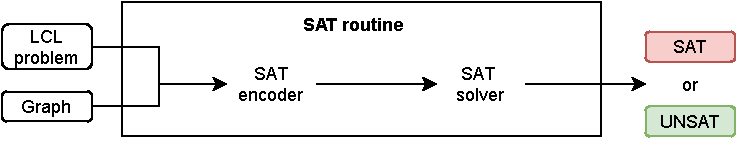
\includegraphics[]{diagrams/implementation_idea_diagram2.pdf}
\caption{The SAT routine. When given a multigraph and an LCL problem, it checks if a valid labeling exists.}
\label{fig:implementation:1}
\end{figure}

We repeat the routine for each multigraph, as shown in the Algorithm \ref{alg:counterexample_finder}, and terminate early if the result is UNSAT.
\todo{WIP}

\begin{figure}[H]
\centering
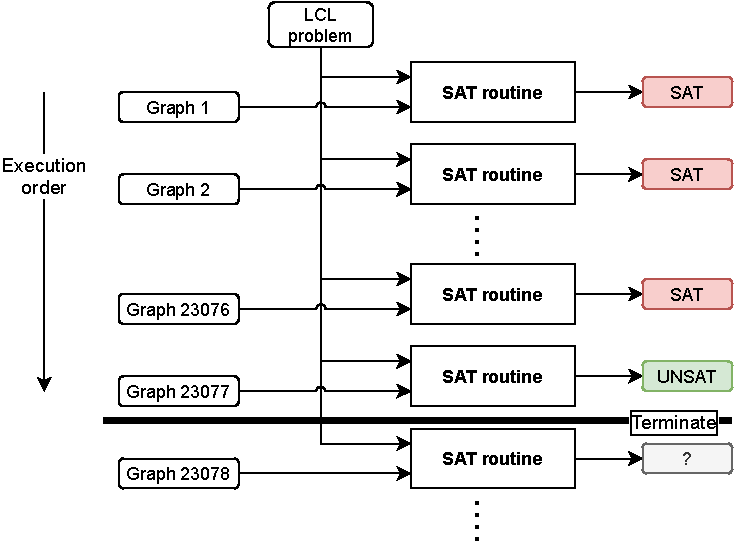
\includegraphics[]{diagrams/implementation_idea_diagram3.pdf}
\caption{An example of an execution of multiple SAT routines. Execution terminates at graph $77$ when first UNSAT is encountered.}
\label{fig:implementation:2}
\end{figure}

%TODO biregular multigraphs?
%TODO LCL problems on biregular trees etc?

%When we assume that an LCL problem $\Pi$ is solvable in PN, we mean that there exists a deterministic distributed algorithm $A$ in PN model, that finds a solution for all multigraphs i.e. algorithm $A$ works in every multigraph.
%Every simple graph is also a multigraph, thus multigraphs are more relaxed in terms of definition.
%Allowing parallel edges potentially gives us counterexamples with smaller graph sizes when we use the increasing strategy i.e. our algorithm might terminate succesfully much earlier with the desired result and graphs do not necessarily become as complex as they would be with only simple graphs.
%%TODO where to discuss about solutions that have been found only with multigraphs? Have we found any solutions with only simple graphs?
%Smaller graphs mean less complexity and less performance required but as there are also more graphs to iterate, it is not so simple to justify allowing parallel edges only with this argument.
%The main argument is that allowing parallel edges gives us more opportunities to find counterexamples.
%It might be that in some problems we cannot even find counterexamples without parallel.

%This is indeed what we have used in this work.
%Probably, we have to iterate a lot of graphs.
%For this purpose we want to be able to generate the graphs.



\subsection{Generating multigraphs}

\subsection{Generating LCL-problems}

\subsection{Boolean satisfiability problem}
\todo{Explain
\begin{itemize}
  \item SAT problems, %TODO
  \item DIMACS CNF, %TODO
  \item SAT solvers, %TODO
\end{itemize}
}

\subsection{SAT solvers} % talk about sats generally before talkign specifically how we encode the problems

\subsection{SAT encoding and solving}

\todo{Use the section 4.1 ``SAT encoding'' from \cite{DBLP:conf/sat/JarvisaloKKK12} as an inspiration for this section. Maybe we will find a nice way to present things?}

%\subsection{Software optimizations
\subsection{Caching}
%TODO pre-computing multigraphs and lcl problems and saving them?

\subsection{parallelization}
%TODO Talk about parallelization here or separately in above sections

